\section{Oxford A0 - Linear Algebra}\footnotetext{\url{https://courses.maths.ox.ac.uk/node/5353}}

\subsection{Sheet 1}

\subsubsection{} % 1
\begin{mdframed}
  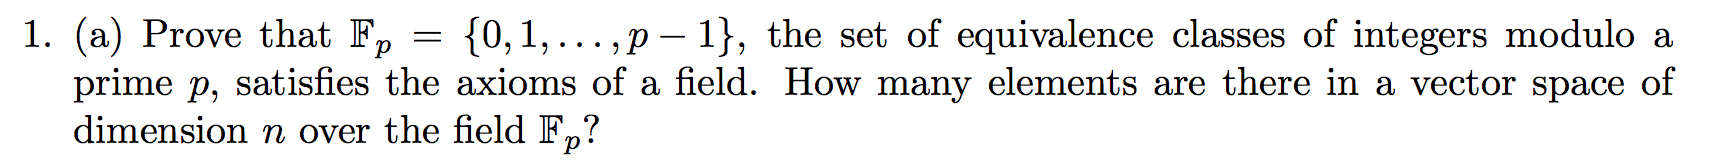
\includegraphics[width=450pt]{img/linear-algebra-a0-1-1-a.png}\\
\end{mdframed}

Let\footnote{Unlike the question, I am trying to use notation that
  distinguishes between integers and their equivalence classes.}
$a, b, c \in \Z$ with $0 \leq a < p, ~~ 0 \leq b < p, ~~ 0 \leq c < p$.

Let $\bar a, \bar b, \bar c \in \F$ be equivalence classes of integers modulo $p$.

The field axioms are listed below, together with proof that they hold for $\F_p$.
\begin{enumerate}
\item \textbf{$\F_p$ is an abelian group under addition}\\
  Define $\bar a + \bar b := \bar{a + b}$, then:
  \begin{enumerate}
  \item \textit{Existence of identity}: $\bar 0$ is the identity since
    $\bar a + \bar 0 = \bar{a + 0} = \bar{a}$ for all $\bar a \in \F_p$.
  \item \textit{Existence of inverses}: $(\bar a)^\1 = \bar{-a}$ since
    $\bar a + \bar{-a} = \bar{a + -a} = \bar{0}$ for all $a \in \F_p$.
  \item \textit{Commutativity}:
    $\bar a + \bar b = \bar{a + b} = \bar{b} + \bar{a}$ for all $a, b \in \F_p$.
  \item \textit{Associativity}:
    $\bar a + (\bar b + \bar c) = \bar a + \bar {b + c} = \bar{a + b + c} =
    \bar{a + b} + \bar{c} = (\bar a + \bar b) + \bar{c}$.
  \end{enumerate}
\item \textbf{$\F_p\setminus\{\bar 0\}$ is an abelian group under multiplication}\\
  Define $\bar a ~ \bar b := \bar{ab}$, then:
  \begin{enumerate}
  \item \textit{Existence of identity}: $\bar 1$ is the identity since
    $\bar a \bar 1 = \bar{a\cdot 1} = \bar{a}$ for all $\bar a \in \F_p$.
    \newpage
  \item \textit{Existence of inverses for everything except additive identity}:\\\\
    The claim is that for all $\bar a \in \F_p \setminus \{\bar 0\}$ there
    exists $\bar b \in \F_p$ such that $\bar a ~ \bar b = \bar 1$.

    \textbf{Proof 1}\\
    We show that elements cannot repeat in a row/column of the group operation
    table, therefore something muct be the inverse.
    \begin{align*}
      a \cdot b &= a \cdot c \mod p\\
      a(b - c) &= 0 \mod p\\
      a &= 0 \text{~or~~} b = c \mod p
    \end{align*}

    \textbf{Proof 2}\\
    Fix an arbitrary $a \in \{1, \ldots, p-1\}$.

    The claim is equivalent to the following: there exists
    $b \in \{0, 1, \ldots, p\}$ such that for all $i, j \in \Z$ there exists
    $k \in \Z$ such that $(ip + a)(jp + b) = kp + 1$.

    But note that $(ip + a)(jp + b) = p(ijp + aj + bi) + ab$ and therefore
    \begin{align*}
      &(ip + a)(jp + b) = kp + 1\\
      \iff &ab = p(k - ijp - aj - bi) + 1.
    \end{align*}
    Since $k$ can be chosen freely, the condition is simply that for all
    $i, j \in \Z$ there exists $k \in \Z$ such that $ab = kp + 1$.

    Note\footnote{I eventually allowed myself to google for a hint here which
      brought up people pointing to Bezout's identity.} that $a$ and $p$ are
    coprime (gcd is 1). By Bezout's identity, there exists $b, -k \in \Z$
    such that
    \begin{align*}
      ba + (-k)p = 1 \iff ab = kp + 1. \qed
    \end{align*}


  \item \textit{Commutativity}:
    $\bar a ~ \bar b = \bar{ab} = \bar{b} ~ \bar{a}$ for all $a, b \in \F_p$.
  \item \textit{Associativity}:
    $\bar a (\bar b \bar c) = \bar a + \bar {bc} = \bar{abc} =
    \bar{ab}~\bar{c} = (\bar a ~ \bar b) \bar{c}$.
  \end{enumerate}
\item \textbf{Distributive axiom}
  \begin{enumerate}
  \item \textit{Multiplication distributes over addition}: $\bar a (\bar b + \bar c) = \bar a (\bar{b + c}) = \bar{a(b+c)} = \bar{ab +
      ac} = \bar{ab} + \bar{ac} = \bar{a}~\bar{b} + \bar{a}~\bar{c}$
  \end{enumerate}
\end{enumerate}

There are $p^n$ elements in a vector space of dimension $n$ over the field $\F_p$.
\newpage
\begin{mdframed}
  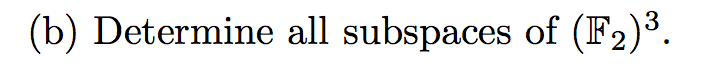
\includegraphics[width=200pt]{img/linear-algebra-a0-1-1-b.png}
\end{mdframed}

\textit{Remark}: This is like the 8 vectors that form the unit cube in
$\R^3$, except that when extended beyond the cube by vector addition or
scalar multiplication they ``wrap around''.

Note that
\begin{align*}
  (\F_2)^3 = \{&\bar 0, \bar 1\}^3\\
           = \{&(\bar 0, \bar 0, \bar 0),\\
               &(\bar 0, \bar 0, \bar 1),\\
               &(\bar 0, \bar 1, \bar 0),\\
               &(\bar 0, \bar 1, \bar 1),\\
               &(\bar 1, \bar 0, \bar 0),\\
               &(\bar 1, \bar 0, \bar 1),\\
               &(\bar 1, \bar 1, \bar 0),\\
               &(\bar 1, \bar 1, \bar 1)\}.
\end{align*}
The set of subspaces of $(\F_2)^3$ is
\begin{align*}
  &\{\{(\bar 0, \bar 0, \bar 0)\}\} ~~~~~~~~~~~~~~~~~~~~~ \cup\\
  &\{\{(\bar 0, \bar 0, \bar 0), x\} ~|~ x \in (\F_2)^3\} ~~~ \cup\\
  &\{\{(\bar 0, a, b) ~|~ a, b \in \F_2\}\}  ~~~~~~~ \cup\\
  &\{\{(a, \bar 0, b) ~|~ a, b \in \F_2\}\}  ~~~~~~~ \cup\\
  &\{\{(a, b, \bar 0) ~|~ a, b \in \F_2\}\}  ~~~~~~~ \cup\\
  &\{(\F_2)^3\}.
\end{align*}

\red{Per AC this is missing, at least, a subspace of size 4. Also see Sylov theorems.}

\newpage
\subsubsection{} % 2
\begin{mdframed}
  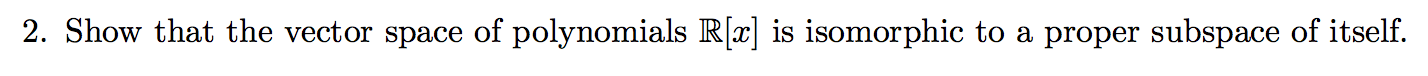
\includegraphics[width=450pt]{img/linear-algebra-a0-1-2.png}\\
\end{mdframed}
We need to:
\begin{enumerate}
\item \textbf{Exhibit a proper subspace $S[x] \subset \R[x]$ and a bijection $f:\R[x] \to S[x]$}\\\\
  Let $a_i \in \R$ for $i = 0, 1, 2, \ldots$ so that
  $\R[x] = \{a_0 + a_1x^1 + a_2x^2 + \ldots\}$.

  Define $S[x] = \{0 + a_1x^1 + a_2x^2 + a_3x^3 + \ldots\}$, i.e. the restriction
  of $\R[x]$ to those polynomials that have constant term zero.

  $S[x]$ is a proper subspace of $\R[x]$ since it contains the zero polynomial,
  and is closed under addition and scalar multiplication.

  Define $f: \R[x] \to S[x]$ where
  $f(a_0 + a_1x^1 + a_2x^2 + \ldots) = 0 + a_0x^1 + a_1x^2 + a_2x^3 + \ldots$.

  $f$ is clearly injective, since if $f(r(x)) = f(r'(x))$ then their
  coefficients $a_0, a_1, \ldots$ are the same and hence $r(x) = r'(x)$.

  Also, $f$ is clearly surjective since if
  $s(x) = a_1x^1 + a_2x^2 + a_3x^3 + \ldots$ then
  $s(x) = f(a_1 + a_2x^1 + a_3x^2 + \ldots)$.

\item \textbf{Prove that $f$ preserves addition}\\\\
  Let $a_i,b_i \in \R$ for $i = 0, 1, 2, \ldots$

  Let $r(x) = a_0 + a_1x^1 + a_2x^2 + \ldots$ and $r'(x) = b_0 + b_1x^1 + b_2x^2 + \ldots$.

  Then
  \begin{align*}
    f\Big(r(x) + r'(x)\Big)
    &= f\Big((a_0 + b_0) + (a_1 + b_1)x^1 + (a_2 + b_2)x^2 + \ldots\Big)\\
    &= 0 + (a_0 + b_0)x^1 + (a_1 + b_1)x^2 + (a_2 + b_2)x^3 + \ldots\\
    &= \Big(0 + a_0x^1 + a_1x^2 + a_2x^3 + \ldots \Big) \\
    &+ \Big(0 + b_0x^1 + b_1x^2 + b_2x^3 + \ldots \Big) \\
    &= f\Big(r(x)\Big) + f\Big(r'(x)\Big).
  \end{align*}

  \begin{align*}
  \end{align*}

\item \textbf{Prove that $f$ preserves scalar multiplication}
  \begin{align*}
    f\Big(\lambda r(x)\Big)
    &= f\Big(\lambda a_0 + \lambda a_1x^1 + \lambda a_2x^2 + \ldots \Big) \\
    &= 0 + \lambda a_0x^1 + \lambda a_1x^2 + \lambda a_2x^3 + \ldots \\
    &= \lambda(0 + a_0x^1 + a_1x^2 + a_2x^3 + \ldots) \\
    &= \lambda f\Big(r(x)\Big)
  \end{align*}


\end{enumerate}

\newpage
\subsubsection{} % 3
\begin{mdframed}
  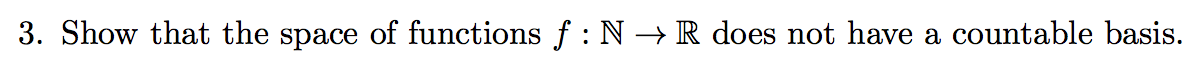
\includegraphics[width=400pt]{img/linear-algebra-a0-1-3.png}\\
\end{mdframed}

Note:
\begin{enumerate}
\item The space of functions $f:\N \to \R$ is the space of real-valued
  infinite sequences.
\item A basis is countable iff a bijection exists between the basis and $\N$.
\end{enumerate}

\red{I haven't managed to do this. What follows is what I was thinking, but
  must be wrong since it contradicts the question.}

Let $x_i \in \R$ for
$i \in \N$ and define the following:
\begin{itemize}
\item $F_n := \{(x_1, x_2, \ldots, x_n) ~|~ x_1, x_2, \ldots, x_n \in \R\}$ is
  the space of functions\\$f:\{1,2, \ldots, n\} \to \R$
\item $F_\infty := \{(x_1, x_2, \ldots) ~|~ x_1, x_2, \ldots \in \R\}$ is the
  space of functions $f:\N \to \R$.
\end{itemize}

Note that $F_1 = \{x_1 ~|~ x_1 \in \R\} = \R$. Therefore every basis for $F_1$ has cardinality
1 (every basis is a set containing a single non-zero real number).

Similarly, $F_2 = \R^2$, and every basis of $F_2$ has cardinality 2.

\red{Basically it seems like the following is a basis of this space of functions,
  but it is countable:}
\begin{align*}
  &(1, 0, 0, \ldots),\\
  &(0, 1, 0, \ldots),\\
  &(0, 0, 1, \ldots),\\
  &\ldots\\
\end{align*}

\red{I think the answer here is that $E$ is a basis for $F_\infty$ iff every
  element of $F_\infty$ can be expressed as a linear combination of a
  \textit{finite} number of elements from $E$. But this is untrue, at least for
  the basis I have suggested, since for example the constant function
  $f(i) = 1 ~\forall i$ fails.}

% ~\\
% \hrule




\newpage
\subsubsection{} % 4
\begin{mdframed}
  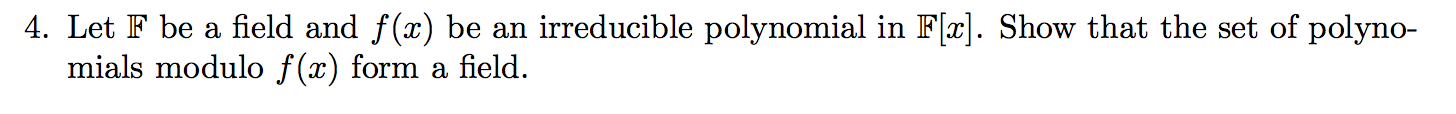
\includegraphics[width=400pt]{img/linear-algebra-a0-1-4.png}\\
\end{mdframed}
Let $P$ be the set of polynomials modulo $f(x)$.

The field axioms are listed below, together with proof that they hold for $P$.
\begin{enumerate}
\item \textbf{$P$ is an abelian group under addition}\\\\
  Define $\bar{g(x)} + \bar{h(x)} := \bar{g(x) + h(x)}$, then:
  \begin{enumerate}
  \item \textit{Existence of identity}:\\
    The additive identity is $\bar 0 = \Big\{f(x)g(x) ~|~ g(x) \in \F[x]\Big\}$.

  \item \textit{Existence of inverses}:\\
    $\bar{g(x)}^{~\1} = \bar{-g(x)}$ for all $g(x) \in P$.
  \item \textit{Commutativity and Associativity}:\\
    Proofs of these are essentially the same as for $\F_p$ (question 1).
  \end{enumerate}
\item \textbf{$P\setminus\{\bar 0\}$ is an abelian group under multiplication}\\\\
  Define $\bar{g(x)} \cdot \bar{h(x)} := \bar{g(x)\cdot h(x)}$, then:
  \begin{enumerate}
  \item \textit{Existence of identity}:\\
    The multiplicative identity is $\bar 1 = \Big\{f(x)g(x) + 1~|~ g(x) \in \F[x]\Big\}$.

  \item \textit{Existence of inverses for everything except additive identity}:\\\\
    The claim is that for all $\bar a \in \F_p \setminus \{\bar 0\}$ there
    exists $\bar b \in \F_p$ such that $\bar a ~ \bar b = \bar 1$.

    Fix an arbitrary $a \in \{1, \ldots, p-1\}$.

    The claim is equivalent to the following: there exists
    $b \in \{0, 1, \ldots, p\}$ such that for all $i, j \in \Z$ there exists
    $k \in \Z$ such that $(ip + a)(jp + b) = kp + 1$.

    But note that $(ip + a)(jp + b) = p(ijp + aj + bi) + ab$ and therefore
    \begin{align*}
      &(ip + a)(jp + b) = kp + 1\\
      \iff &ab = p(k - ijp - aj - bi) + 1.
    \end{align*}
    Since $k$ can be chosen freely, the condition is simply that for all
    $i, j \in \Z$ there exists $k \in \Z$ such that $ab = kp + 1$.

    Note\footnote{I eventually allowed myself to google for a hint here which
      brought up people pointing to Bezout's identity.} that $a$ and $p$ are
    coprime (gcd is 1). By Bezout's identity, there exists $b, -k \in \Z$
    such that
    \begin{align*}
      ba + (-k)p = 1 \iff ab = kp + 1. \qed
    \end{align*}


  \item \textit{Commutativity}:
    $\bar a ~ \bar b = \bar{ab} = \bar{b} ~ \bar{a}$ for all $a, b \in \F_p$.
  \item \textit{Associativity}:
    $\bar a (\bar b \bar c) = \bar a + \bar {bc} = \bar{abc} =
    \bar{ab}~\bar{c} = (\bar a ~ \bar b) \bar{c}$.
  \end{enumerate}
\item \textbf{Distributive axiom}
  \begin{enumerate}
  \item \textit{Multiplication distributes over addition}: $\bar a (\bar b + \bar c) = \bar a (\bar{b + c}) = \bar{a(b+c)} = \bar{ab +
      ac} = \bar{ab} + \bar{ac} = \bar{a}~\bar{b} + \bar{a}~\bar{c}$
  \end{enumerate}
\end{enumerate}

\newpage

\begin{mdframed}
  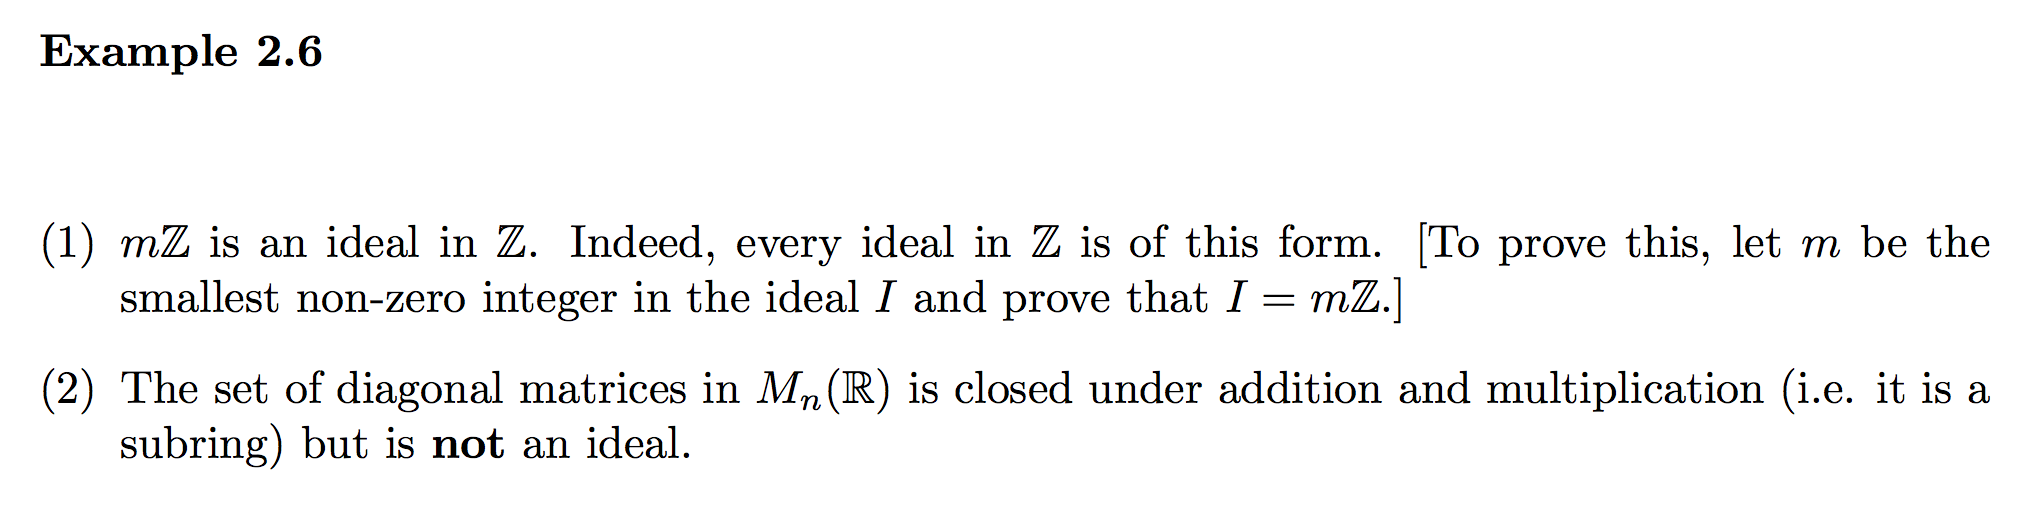
\includegraphics[width=400pt]{img/linear-algebra-eg-2-6.png}
\end{mdframed}

\begin{claim*}
  $m\Z$ is an ideal in $\Z$.
\end{claim*}

\begin{proof}Let $s, t \in m\Z$ and $i, j, k \in \Z$.

  Then $s = mi$ and $t = mj$ for some $i, j$.

  Therefore $s - t = m(i - j) \in m\Z$ and $ks = sk = m(ki) \in m\Z$.
\end{proof}

\begin{claim*}
  Every ideal in $\Z$ is of the form $m\Z$.
\end{claim*}

\begin{proof}
  Let $I$ be an ideal in $\Z$ and let $m$ be the smallest non-zero positive integer in $I$.

  % Let $i \in I$. We have that $i - m \in I$ and that $mi \in I$.

  % We want to show that $i \in m\Z$.

  Let $i \in I$. We want to show that $i \in m\Z$.

  We have:

  $ki \in I$ for all $k \in \Z$.

  $i - j \in I$ for all $j \in I$.

  $i - m \in I$.


  % By the definition of an ideal, $ki \in I$ for
  % all $k \in \Z$. Therefore $i$ is a multiple of $m$.

  % Conversely, suppose $i \in m\Z$. We want to show that $i \in I$.


  % is a multiple of $m$. So $i = km$ for some $k \in \Z$.
\end{proof}


\newpage
\subsubsection{} % 5
\begin{mdframed}
  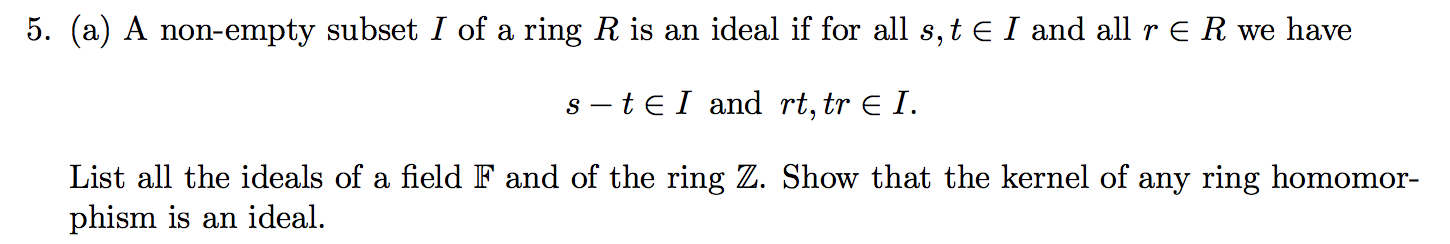
\includegraphics[width=400pt]{img/linear-algebra-a0-1-5-a.png}\\
\end{mdframed}

The set of ideals of a field $\F$ is $\{a\F ~|~ a \in \F\} = \{\{0\}, \F\}$.

The set of ideals of the ring $\Z$ is $\{m\Z ~|~ m \in \Z\}$.


\begin{definition*}
  Let $R, S$ be rings and let $r_1, r_2 \in R$. A \emph{ring homomorphism} is $f:R \to S$ such that
  $f(r_1 + r_2) = f(r_1) + f(r_2)$ and $f(r_1r_2) = f(r_1)f(r_2)$.
\end{definition*}

\begin{claim*}
  The kernel of any ring homomorphism is an ideal.
\end{claim*}

\begin{proof}
  Let $H$ be the kernel of a ring homomorphism $f:R \to S$, and let

  We want to show that
  \begin{enumerate}
  \item $h_1 - h_2 \in H$ for all $h_1, h_2 \in H$, and \label{ring-hom-ideal-1}
  \item $rh \in H$ for all $r \in R, h \in H$. \label{ring-hom-ideal-2}
  \end{enumerate}

  We have $f(h_1 - h_2) = f(h_1) + f(-h_2) = f(h_1) - f(h_2) = 0 - 0 = 0$, proving
  (\ref{ring-hom-ideal-1}).

  And $f(rh) = f(r)f(h) = f(r)\cdot 0 = 0$, proving (\ref{ring-hom-ideal-2}).

\end{proof}



\newpage
\begin{mdframed}
  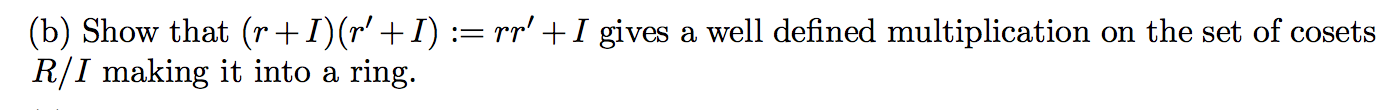
\includegraphics[width=400pt]{img/linear-algebra-a0-1-5-b.png}\\
\end{mdframed}

\begin{mdframed}
  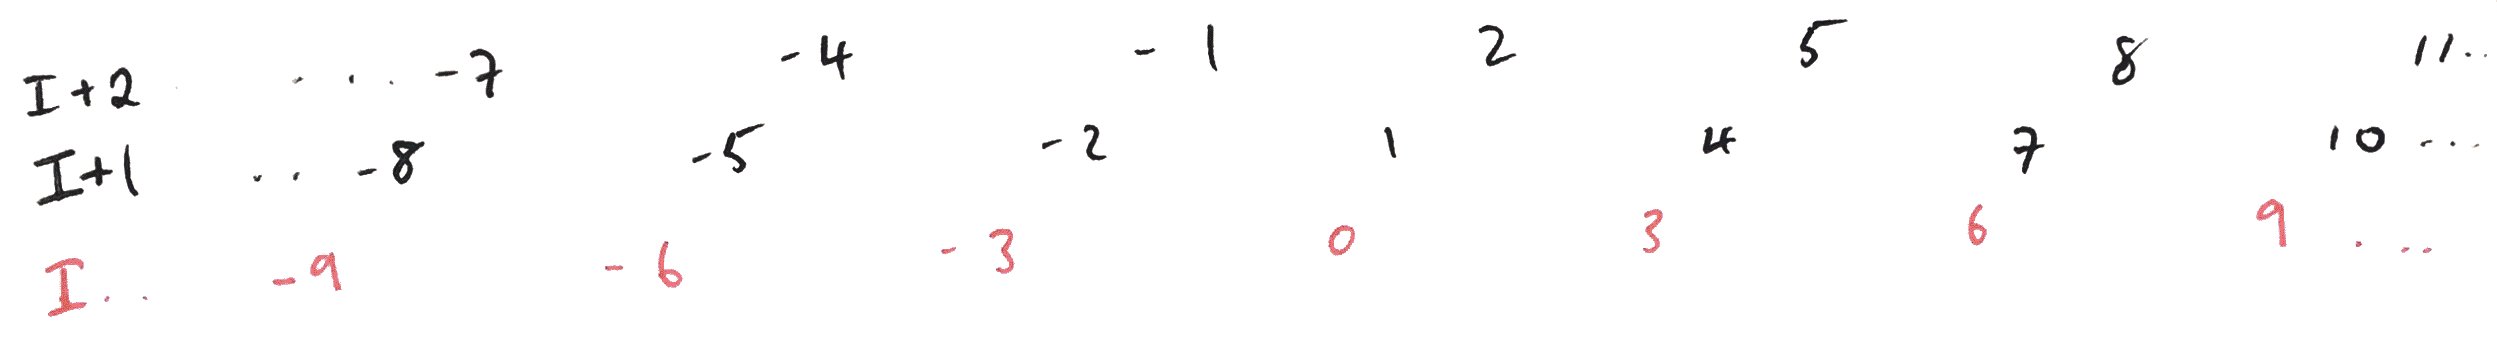
\includegraphics[width=400pt]{img/ideal-in-integers.png}
\end{mdframed}

\begin{mdframed}
  \begin{remark*}
    Recall that in group theory a quotient group is formed by:
    \begin{enumerate}
    \item Identify a subgroup.
    \item Form cosets.
    \item Inherit operation on cosets from operation on original group elements.
    \end{enumerate}
    But only if the subgroup is normal.

    Here, the ideal $I$ is playing the role of subgroup.~\\
  \end{remark*}
\end{mdframed}

Let $S$ and $T$ be cosets, and let $r \in S$ and $r' \in T$. We need to show that $rr' + I$ is the
same coset, for all choices of $r$, $r'$.

\newpage
\begin{mdframed}
  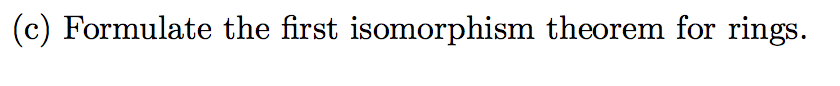
\includegraphics[width=280pt]{img/linear-algebra-a0-1-5-c.png}\\
\end{mdframed}

\newpage
\subsubsection{} % 6
\begin{mdframed}
  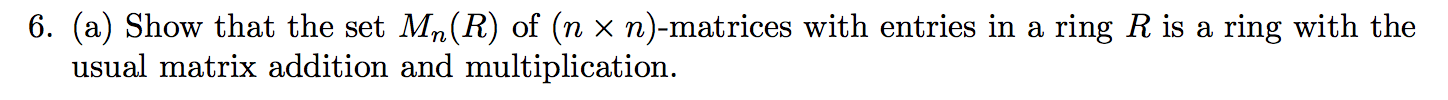
\includegraphics[width=400pt]{img/linear-algebra-a0-1-6-a.png}\\
\end{mdframed}
It is an abelian group under addition since:
\begin{enumerate}
\item The zero matrix is the additive identity.
\item For all $r \in R$, we have $-r \in R$. Therefore for $A \in M_n(R)$ we have $-A \in M_n(R)$.
\item It is closed (result is a matrix of same dimension).
\item Addition commutes.
\end{enumerate}

Under multiplication:
\begin{enumerate}
\item It is closed because addition and multiplication in the ring are closed.
\item Multiplication is associative.
\item Both distributive laws hold ($A(B + C) = AB + AC$ and $(B + C)A = BA + CA$.)
\end{enumerate}

Therefore it is a ring (but not a field since multiplicative inverses may not exist).

\begin{mdframed}
  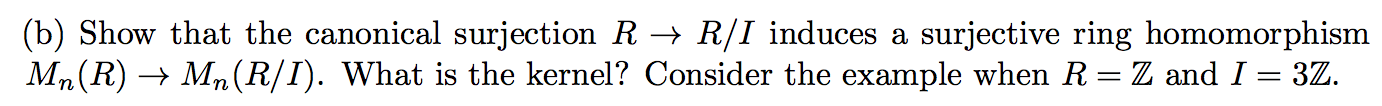
\includegraphics[width=400pt]{img/linear-algebra-a0-1-6-b.png}\\
\end{mdframed}
Let $I$ be an ideal of a ring $R$.

Note that:
\begin{enumerate}
\item If $r$ is an entry in a matrix $A \in M_n(R)$ then $r \in R$.
\item If $s$ is an entry in a matrix $\Gamma \in M_n(R/I)$ then $s \in R/I$ is a coset.
\end{enumerate}

The ``canonical surjection'' $R \to R/I$ is defined by $r \mapsto rI$.

It induces a map $f:M_n(R) \to M_n(R/I)$ defined by $A \mapsto \Gamma$, where
$\Gamma_{ij} = A_{ij}I$ for all $i,j \in \{1, \ldots, n\}$.

Let $A, B \in M_n(R)$.

Then
\begin{align*}
  \Big(f(A + B)\Big)_{ij}
  &= (A_{ij} + B_{ij})I ~~~~~~~~~~~~~~~~~~~\text{(by definition of the induced map)}\\
  &= A_{ij}I + B_{ij}I ~~~~~~~~~~~~~~~~~~~~\text{(by definition of addition on the cosets)}\\
  &= \Big(f(A)\Big)_{ij} + \Big(f(B)\Big)_{ij} ~~~~~~~\text{(by definition of the induced map)}\\
  &= \Big(f(A) + f(B)\Big)_{ij}~~~~~~~~~~~~~\text{(by definition of matrix addition)},\\
\end{align*}

and

\begin{align*}
  \Big(f(AB)\Big)_{ij}
  &= (AB)_{ij}I ~~~~~~~~~~~~~~~~~~~\text{(by definition of the induced map)}\\
  &= \sum_k A_{ik}B_{kj}I\\
  &= \sum_k (A_{ik}I)(B_{kj}I)\\
  &= \Big(f(A)f(B)\Big)_{ij}.
\end{align*}

Therefore $f$ preserves the additive and multiplicative structure on $M_n(R)$.

\red{TODO: show it is surjective}

The additive identity in $M_n(R/I)$ is the matrix containing $I$ in every entry.

The kernel is the set of matrices that get mapped to the (additive) identity in $M_n(R/I)$.

Therefore the kernel is $\{A ~|~ A_{ij} \in I ~\forall~ i, j \in \{1, \ldots, n\}\}$.

For example, suppose $R = \Z$ and $I = 3\Z$.

Then $R/I = \{3\Z, 3\Z + 1, 3\Z + 2\}$.

The kernel is $\{A ~|~ A_{ij} \in 3\Z\}$.

\begin{mdframed}
  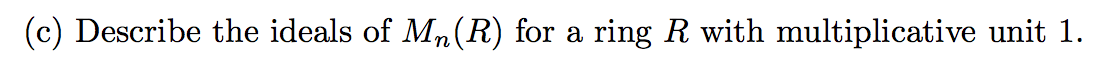
\includegraphics[width=350pt]{img/linear-algebra-a0-1-6-c.png}\\
\end{mdframed}
The set of diagonal matrices is the sole ideal?

\newpage
\subsubsection{} % 7
\begin{mdframed}
  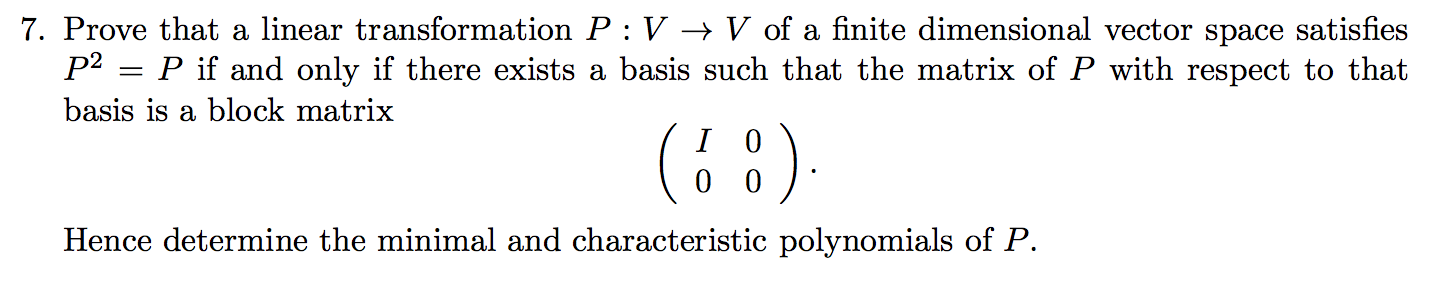
\includegraphics[width=400pt]{img/linear-algebra-a0-1-7.png}\\
\end{mdframed}

\subsubsection{} % 8
\begin{mdframed}
  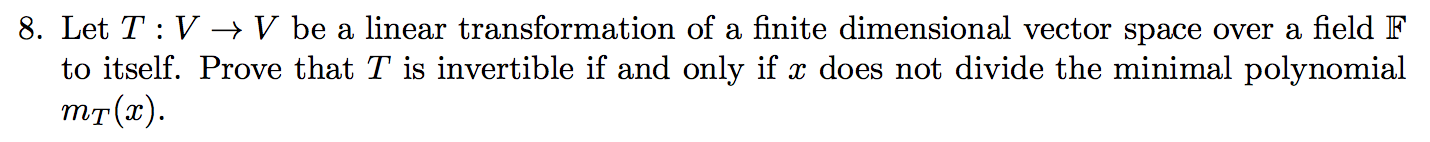
\includegraphics[width=400pt]{img/linear-algebra-a0-1-8.png}\\
\end{mdframed}

\subsubsection{} % 9
\begin{mdframed}
  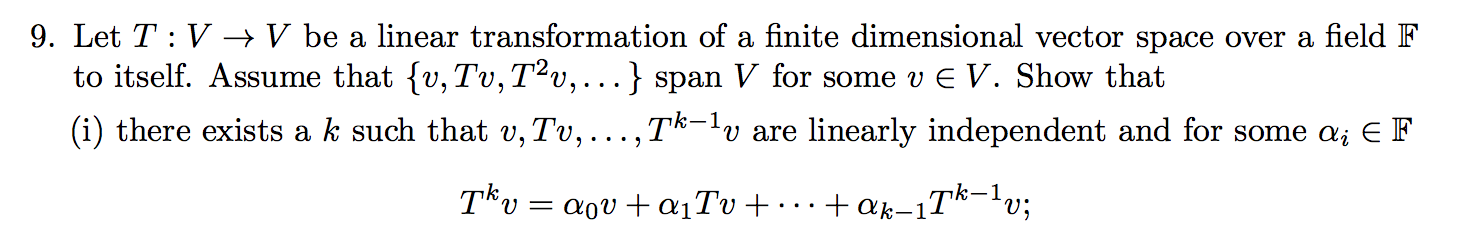
\includegraphics[width=400pt]{img/linear-algebra-a0-1-9-a.png}\\
\end{mdframed}
\begin{mdframed}
  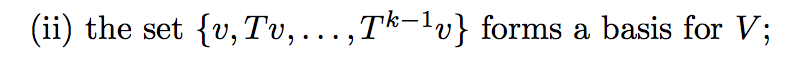
\includegraphics[width=250pt]{img/linear-algebra-a0-1-9-b.png}\\
\end{mdframed}
\begin{mdframed}
  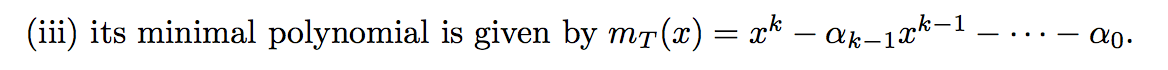
\includegraphics[width=350pt]{img/linear-algebra-a0-1-9-c.png}\\
\end{mdframed}
\begin{mdframed}
  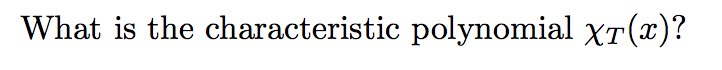
\includegraphics[width=220pt]{img/linear-algebra-a0-1-9-d.png}\\
\end{mdframed}

\newpage
\subsection{Sheet 2}

% https://math.stackexchange.com/questions/555726/inducing-a-linear-map-on-quotient-spaces
\begin{mdframed}
  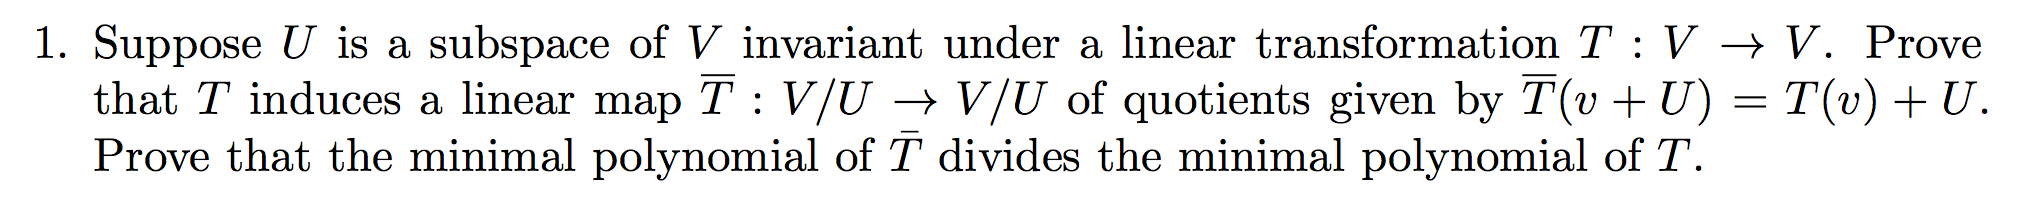
\includegraphics[width=400pt]{img/linear-algebra-a0-2-1.png}
\end{mdframed}
\begin{mdframed}
  \begin{example*}
    Let $V = \R^3$, $U$ be a one-dimensional subspace, and $T$ be rotation around the axis
    $U$. Choose an orthonormal basis $\{w, v, u\}$ for $\R^3$ where $u \in U$. Then the matrix
    of $T$ is
    \begin{align*}
      \matMMMxNNN
      {\cos\theta}{-\sin\theta}{0}
      {\sin\theta}{~~\cos\theta}{0}
      {0}         {           0}{1}.
    \end{align*}

    $V/U$ is the set of lines parallel to $U$. $U$ is the kernel of a projection onto $\R^2$, and
    $V/U \cong \R^2$.

    ``In some sense'' the matrix of $\bar T:V/U \to V/U$ is the block
    $\matMMxNN{\cos\theta}{-\sin\theta}
    {\sin\theta}{~~\cos\theta}$.
  \end{example*}
\end{mdframed}

Let $v + U$ be a coset of $U$. Then the induced mapping is given by
\begin{align*}
  \bar T(v + U) &= \{T(v + u) ~|~ u \in U\}\\
                &= \{T(v) + T(u) ~|~ u \in U\}\\
                &= T(v) + T(U)\\
                &= T(v) + U.
\end{align*}

\begin{claim*}
  $\bar T$ is a linear map.
\end{claim*}

\begin{proof}~\\
  \red{TODO: is there any question about it being well-defined?}

  Vector addition:
  \begin{align*}
    \bar T\Big((v + U) + (w + U)\Big)
    &= \bar T\Big((v + w) +  U\Big) ~~~~~~~~~~~~~\text{(by definition of addition on quotient group)}\\
    &= T(v + w) + U              ~~~~~~~~~~~~~~~~~\text{(by definition of $\bar T$)}\\
    &= (T(v) + T(w)) + U              ~~~~~~~~~~\text{(by linearity of $T$)}\\
    &= (T(v) + U) + (T(w) + U) ~~\text{(by definition of addition on quotient group)}\\
    &= \bar T(v + U) + \bar T(w + U)              ~~~~~~~\text{(by definition of $\bar T$)}
  \end{align*}
  Multiplication by a scalar $\lambda \in \F$:
  \begin{align*}
    \bar T\Big(\lambda(v + U)\Big)
    &= \bar T\Big(\lambda v + \lambda U\Big) ~~\text{(by (scalar)(SetOfVectors) and (vector) + (SetOfVectors) syntax)}\\
    &= T(\lambda v) + \lambda U~~~~\text{(by definition of $\bar T$)}\\
    &= \lambda T(v) + \lambda U~~~~\text{(by linearity of $T$)}\\
    &= \lambda\Big(T(v) + U\Big)  ~~\text{(by (scalar)(SetOfVectors) and (vector) + (SetOfVectors) syntax)}\\
    &= \lambda \bar T(v + U)~~~~~\text{(by definition of $\bar T$)}
  \end{align*}
\end{proof}

\begin{definition*}[Minimal polynomial]
  Let $V$ be a finite-dimensional vector space over $\F$, and let $A$ be a matrix of a linear
  transformation $T:V \to V$.

  The \emph{minimal polynomial} $m_A(x)$ is the monic polynomial $p(x)$ of minimal degree such that
  $p(A) = 0$.
\end{definition*}

\begin{lemma*}~\\
  \begin{enumerate}
  \item The minimal polynomial exists for any endomorphic linear transformation.
  \item The minimal polynomial is unique.
  \item Let $f(x)$ be a polynomial. If $f(A) = 0$ then $m_A | f$.
  \end{enumerate}
\end{lemma*}

\begin{claim*}
  The minimal polynomial of $\bar T$ divides the minimal polynomial of $T$.
\end{claim*}

\begin{proof} (I)\\

  \begin{align*}
    m_T(\bar T)
  \end{align*}

  $\vdots$

  We have $m_T(\bar T) = 0$, therefore $m_{\bar T}| m_T$.

\end{proof}

\begin{proof} (II)\\
  Let $J = \dim U$ and $K = \dim V$.

  Pick a basis of $U$ and extend it to a basis $\mathcal B$ of $V$.

  Order the elements of the basis $\mathcal B$ such that the last $J$ elements are the basis of
  $U$.

  Let $A$ be the matrix of $T$ with respect to $\mathcal B$.

  Then, since $U$ is invariant under $T$, $A$ has a block structure
  \begin{align*}
    A = \matMMxNN{~\bar A}{0}
                 {~0     }{B}.
  \end{align*}

  Claim: $\bar A$ is the matrix of $\bar T$ with respect to some basis of $V/U$.

  Note that
  \begin{align*}
    \lambda A^n = \matMMxNN{~\lambda{\bar A}^n}{0}
                            {~0      }{\lambda B^n}.
  \end{align*}
  Let $p(x)$ be a polynomial. Then $p(A) = 0 \implies p(\bar A) = 0$.

  Let $m_A(x)$ and $m_{\bar A}(x)$ be the minimal polynomials of $A$ and $\bar A$ respectively.

  By definition, $m_A(A) = 0$.

  Therefore $m_A(\bar A) = 0$, therefore $m_{\bar A}| m_A$.

  Equivalently, $m_{\bar T}| m_T$.
\end{proof}


% \newpage
\begin{mdframed}
  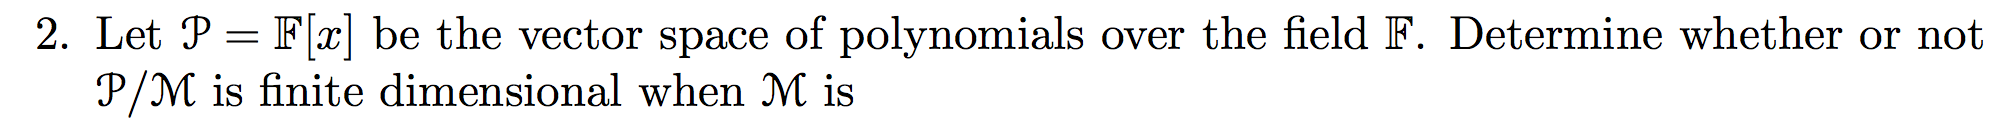
\includegraphics[width=400pt]{img/linear-algebra-a0-2-2.png}
\end{mdframed}
\begin{mdframed}
  
\includegraphics[width=400pt]{img/linear-algebra-a0-2-2-1.png}
\end{mdframed}

Let $D^n:\mc P \to \mc P$ be the $n$-th derivative operator.

Then $\mc P_n$ is the kernel of $D^{n+1}$.

Furthermore, $D^n$ is a homomorphism (preserves addition of polynomials).

By the First Isomorphism Theorem, $\mc P/\mc P_n \cong \Im D^{n+1}$.

\begin{claim*}
  $\Im D^n = \mc P$ (surjective) for all $n \in \N$.
\end{claim*}

\begin{proof}
  Let $p(x) = \sum_{i=1}^k\lambda_ix^i \in \mc P$. Then
  $D^n \Big(x^n\sum_{i=1}^k\frac{\lambda_i}{(i>+n)_{(n)}}x^i\Big) = p(x)$, so $D^n$ is surjective.
\end{proof}

Therefore $\mc P/\mc P_n \cong \mc P$.

Therefore $\mc P/\mc P_n$ is infinite-dimensional.

\begin{remark*}
  Each element of $\mc P/\mc P_n$ is a set of polynomials differing only by additive terms
  of degree $n$ or less.
\end{remark*}

\begin{mdframed}
  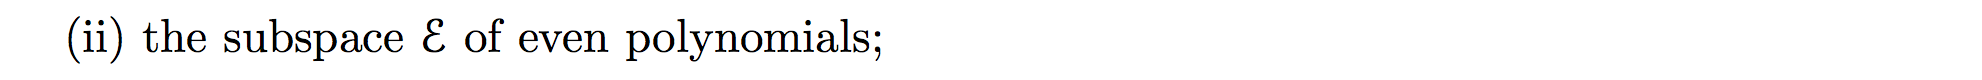
\includegraphics[width=400pt]{img/linear-algebra-a0-2-2-2.png}
\end{mdframed}
Let $\mc E$ and $\mc O$ be the set of even and odd polynomials respectively.

Let $f:\mc P \to \mc P$ be given by $p(x) := $ (the odd terms of $p(x)$).

Then $\Im f = \mc O$ and $\Ker f = \mc E$.

Therefore $\mc P/\mc E \cong \mc O$, infinite-dimensional.


\begin{mdframed}
  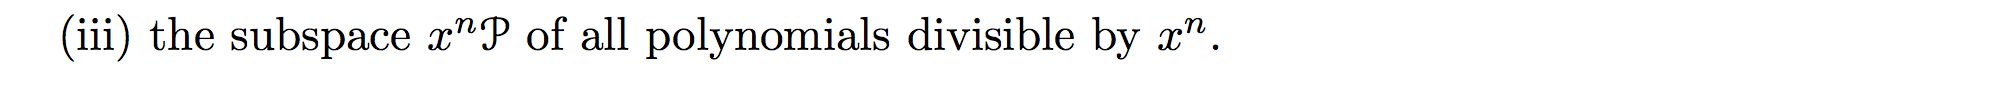
\includegraphics[width=400pt]{img/linear-algebra-a0-2-2-3.png}
\end{mdframed}
Let $f: \mc P \to \mc P$ be given by $f(p(x)) := $ (remainder after division by $x^n$).

\begin{claim*}
  $f$ is a homomorphism: $f(p(x) + q(x)) = f(p(x)) + f(q(x))$.
\end{claim*}

Note that $x^n\mc P$ is the kernel of $f$.

\begin{claim*}
  $\Im f = \mc P_{n-1}$.
\end{claim*}

\red{TODO: prove or disprove}.

If these claims are true, then $\mc P/x^n\mc P \cong \mc P_n$, finite-dimensional.

\begin{mdframed}
  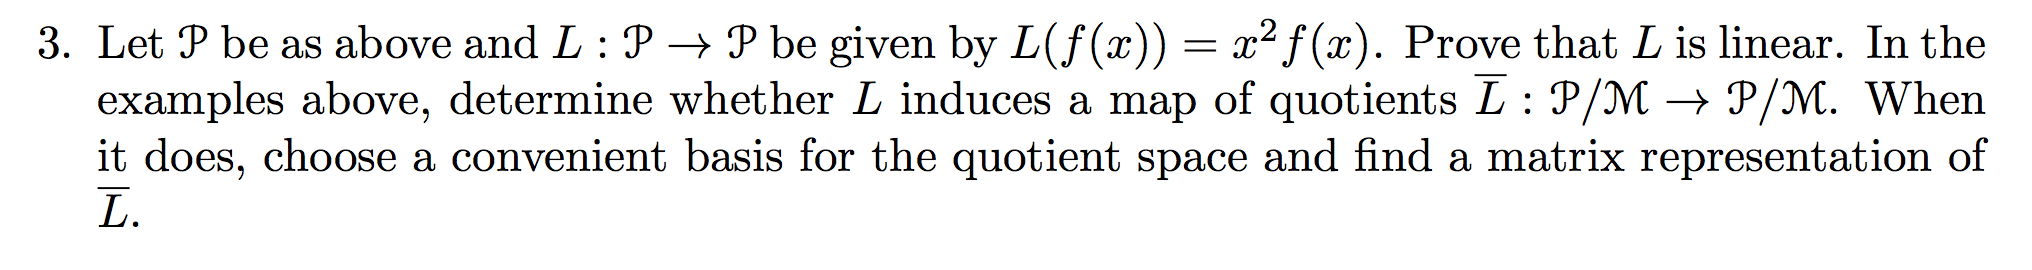
\includegraphics[width=400pt]{img/linear-algebra-a0-2-3.png}
\end{mdframed}

\begin{claim*}
  $L$ is linear.
\end{claim*}

\begin{proof} Note that multiplication of polynomials distributes over addition:
  \begin{align*}
    \Big(\sum_{i=0}^k a_ix^i\Big)\Big(\sum_{i=0}^k b_ix^i + \sum_{i=0}^k c_ix^i\Big)
    &= \Big(\sum_{i=0}^k a_ix^i\Big)\Big(\sum_{i=0}^k (b_i + c_i)x^i\Big)\\
    &= \Big(\sum_{i=0}^{k}\sum_{j=0}^k a_i(b_j + c_j)x^{i+j}\Big)\\
    &= \Big(\sum_{i=0}^{k}\sum_{j=0}^k a_ib_jx^{i+j}\Big) +
       \Big(\sum_{i=0}^{k}\sum_{j=0}^k a_ic_jx^{i+j}\Big)\\
    &= \Big(\sum_{i=0}^k a_ix^i\Big)\Big(\sum_{i=0}^k b_ix^i\Big) +
       \Big(\sum_{i=0}^k a_ix^i\Big)\Big(\sum_{i=0}^k c_ix^i\Big).
  \end{align*}
  Therefore
  \begin{align*}
    L(af(x) + bg(x)) &= x^2(af(x) + bg(x))\\
                     &= ax^2f(x) + bx^2g(x)\\
                     &= aL(f(x)) + bL(g(x)),
  \end{align*}
  where $a, b \in \F$.
\end{proof}

\newpage
\begin{mdframed}
  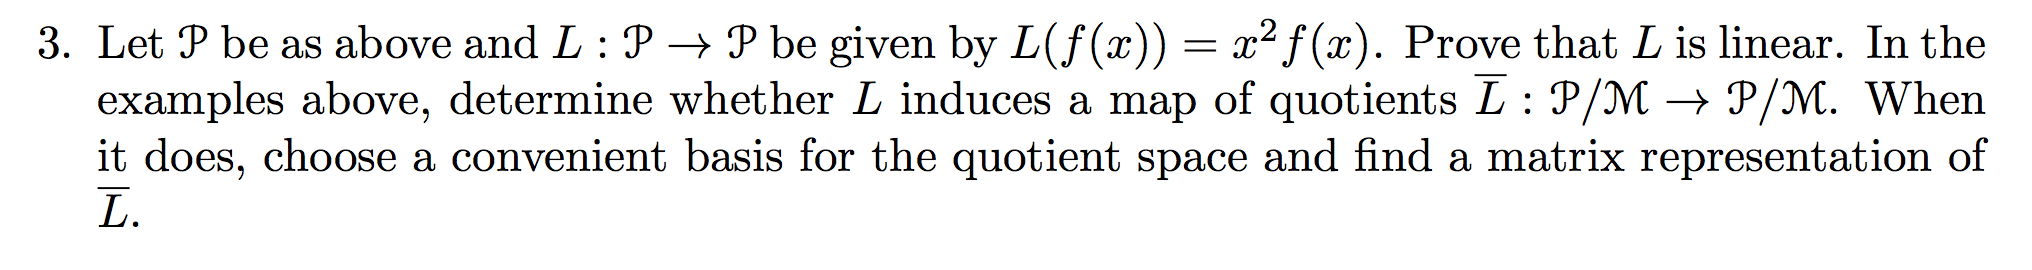
\includegraphics[width=400pt]{img/linear-algebra-a0-2-3.png}
\end{mdframed}

First, a theorem and a corollary:

\begin{theorem*}
  Let $L:V \to W$ be an isomorphism\footnote{note: not linear; but why not homomorphism?} between
  vector spaces $V$ and $W$, and let $A \subseteq V, B \subseteq W$ be subspaces. Then the formula
  $\bar L(v + A) = L(v) + B$ gives a well-defined linear map $\bar L:V/A \to W/B$ if and only if
  $L(A) \subseteq B$.
\end{theorem*}

Therefore

\begin{corollary*}
  Let $L:V \to V$ with $U$ a subspace of $V$. Then $L$ induces a linear map of quotients
  $\bar L:V/U \to V/U$ given by $v + U \mapsto L(v) + U$ if and only if $U$ is invariant under $T$.
\end{corollary*}

~\\

\begin{mdframed}
  
\includegraphics[width=400pt]{img/linear-algebra-a0-2-2-1.png}
\end{mdframed}

% Recall that:
% \begin{enumerate}
% \item $\mc P_n$ is the kernel of $D^{(n+1)}$.
% \item Every coset $\Big(p(x) + \mc P_n\Big) \in \mc P/\mc P_n$ is a set of polynomials differing
%   only by additive terms of degree $n$ or less.
% \end{enumerate}

Note that $L(\mc P_n) = x^2\mc P_n = \mc P_{n+2} \not\subseteq \mc P_n$.

Therefore the formula
\begin{align*}
  \bar L\Big(p(x) + \mc P_n\Big) := x^2p(x) + \mc P_n
\end{align*}
does not give a well-defined map $\bar L:\mc P/\mc P_n \to \mc P/\mc P_n$.

\begin{mdframed}
  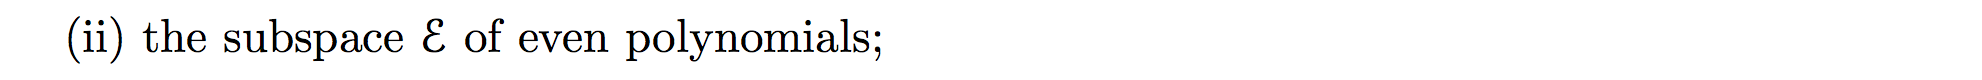
\includegraphics[width=400pt]{img/linear-algebra-a0-2-2-2.png}
\end{mdframed}

% Recall that:
% \begin{enumerate}
% \item $\mc P/\mc E \cong \mc O$, infinite-dimensional.
% \item Every coset is of the form $o(x) + \mc E$, for some odd polynomial $o(x) \in \mc O$.
% \end{enumerate}

Note that $L(\mc E) = x^2\mc E = \mc E$. Therefore the formula
\begin{align*}
  \bar L\Big(p(x) + \mc E\Big) := x^2p(x) + \mc E
\end{align*}
does give a well-defined linear map of quotients $\bar L:\mc P/\mc E \to \mc P/\mc E$.

A basis for $\mc E$ is $\{1, x^2, x^4, \ldots\}$.

To extend this basis to a basis for $\mc P$ we can add the elements of $\{x, x^3, x^5, \ldots\}$.

Therefore (theorem) a basis for $\mc P/\mc E$ is $\{x + \mc E, x^3 + \mc E, x^5 + \mc E, \ldots\}$.

However, the quotient space $\mc P/\mc E \cong \mc O$ is infinite-dimensional and therefore
$\bar L$ has no matrix representation.

% \begin{mdframed}
%   \begin{remark*}
%     Note that $\mc E$ is not in the basis since it is the additive identity in $\mc P/\mc E$: Let 0
%     be the additive identity in the field $\F$. Then
%     $\mc E = 0(x + \mc E) + 0(x^3 + \mc E) + \ldots$. This is true since in general
%     $0\vec v = (1 - 1)\vec v = \vec v - \vec v = \vec 0$.
%   \end{remark*}
% \end{mdframed}

% Since the quotient space is infinite-dimensional, $\bar L$ has no finite matrix representation.

% As an ``infinite matrix'' it would be
% \begin{align*}
%   \begin{pmatrix}
%     0      & 0      & 0      & \cdots\\
%     1      & 0      & 0      & \cdots\\
%     0      & 1      & 0      & \cdots\\
%     \vdots & \vdots & \vdots & \ddots
%   \end{pmatrix},
% \end{align*}
% that is, an infinite-dimensional identity matrix below a row of zeros.

\begin{mdframed}
  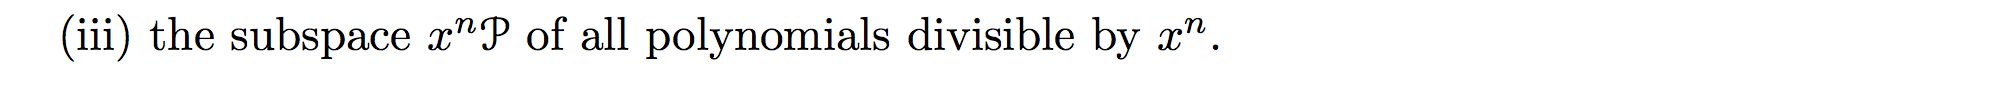
\includegraphics[width=400pt]{img/linear-algebra-a0-2-2-3.png}
\end{mdframed}

% Recall that:
% \begin{enumerate}
% \item $x^n\mc P$ is the kernel of the homomorphism which sends $p(x) \in \mc P$ to its remainder
%   after division by $x^n$. The image is $\mc P_{n-1}$.
% \item Therefore $\mc P/x^n\mc P \cong \mc P_{n-1}$, finite-dimensional.
% \item Every coset is of the form $p(x) + x^n\mc P$.
% \end{enumerate}

Note that $L(x^n\mc P) = x^{n+2}\mc P \subseteq x^n\mc P$.

Therefore the formula
\begin{align*}
  \bar L\Big(p(x) + x^n\mc P\Big) := x^2p(x) + x^n\mc P.
\end{align*}
gives a well-defined linear map of quotients.

A basis for $\mc P$ is $\{1, x, x^2, \ldots\}$.

A basis for $x^n\mc P$ is $\{x^n, x^{n+1}, \ldots\}$.

Therefore (theorem) a basis for the quotient space $\mc P/x^n\mc P$ is
\begin{align*}
  \{1 + x^n\mc P, x + x^n\mc P, x^2 + x^n\mc P, \ldots, x^{n-1} + x^n\mc P\}.
\end{align*}

A matrix representation for $\bar L$ with respect to this basis is
\begin{align*}
  [\vec a_1, \vec a_2, \ldots, \vec a_{n-1}],
\end{align*}
where $\vec a_{j}$ is a column vector with 1 in its $(j + 2)$-th entry, and 0 elsewhere.
